\subsection{Entrant al concepte del Cub de Rubik}

\subsubsection{Error a l'interpretar el concepte del cub}

Una gran majoria de la població ha tingut a les seves mans un cub de Rubik, i han intentat resoldre'l sense èxit. Això és totalment normal, ja que només el saben resoldre un 5,8\% de les persones que ho han intentat\cite{redbull-cub}.
\\ \\Aquesta xifra es sol atribuir a la dificultat del cub, però després d'aprendre a fer el cub de rubik t'adones compte de què la raó no és aquesta. El fracàs a l'hora trobar la solució bé donat pel fet d'interpretar malament el concepte del funcionament del cub.
\\ \\La majoria de les persones es pensa que el cub conté 54 "peces" de colors perquè calculen que per cada cara hi ha 9 peces i en un cub hi ha 6 cares, per tant estan treballant color a color.
\\ \\La manera correcta d'interpretar el cub és pensar en el funcionament, com si el desmuntessis, ja que consta de 12 arestes i 8 cantonades, a més a més dels 6 centres que no es poden moure i que per tant no es compten.

\begin{figure}[h]
    \centering
    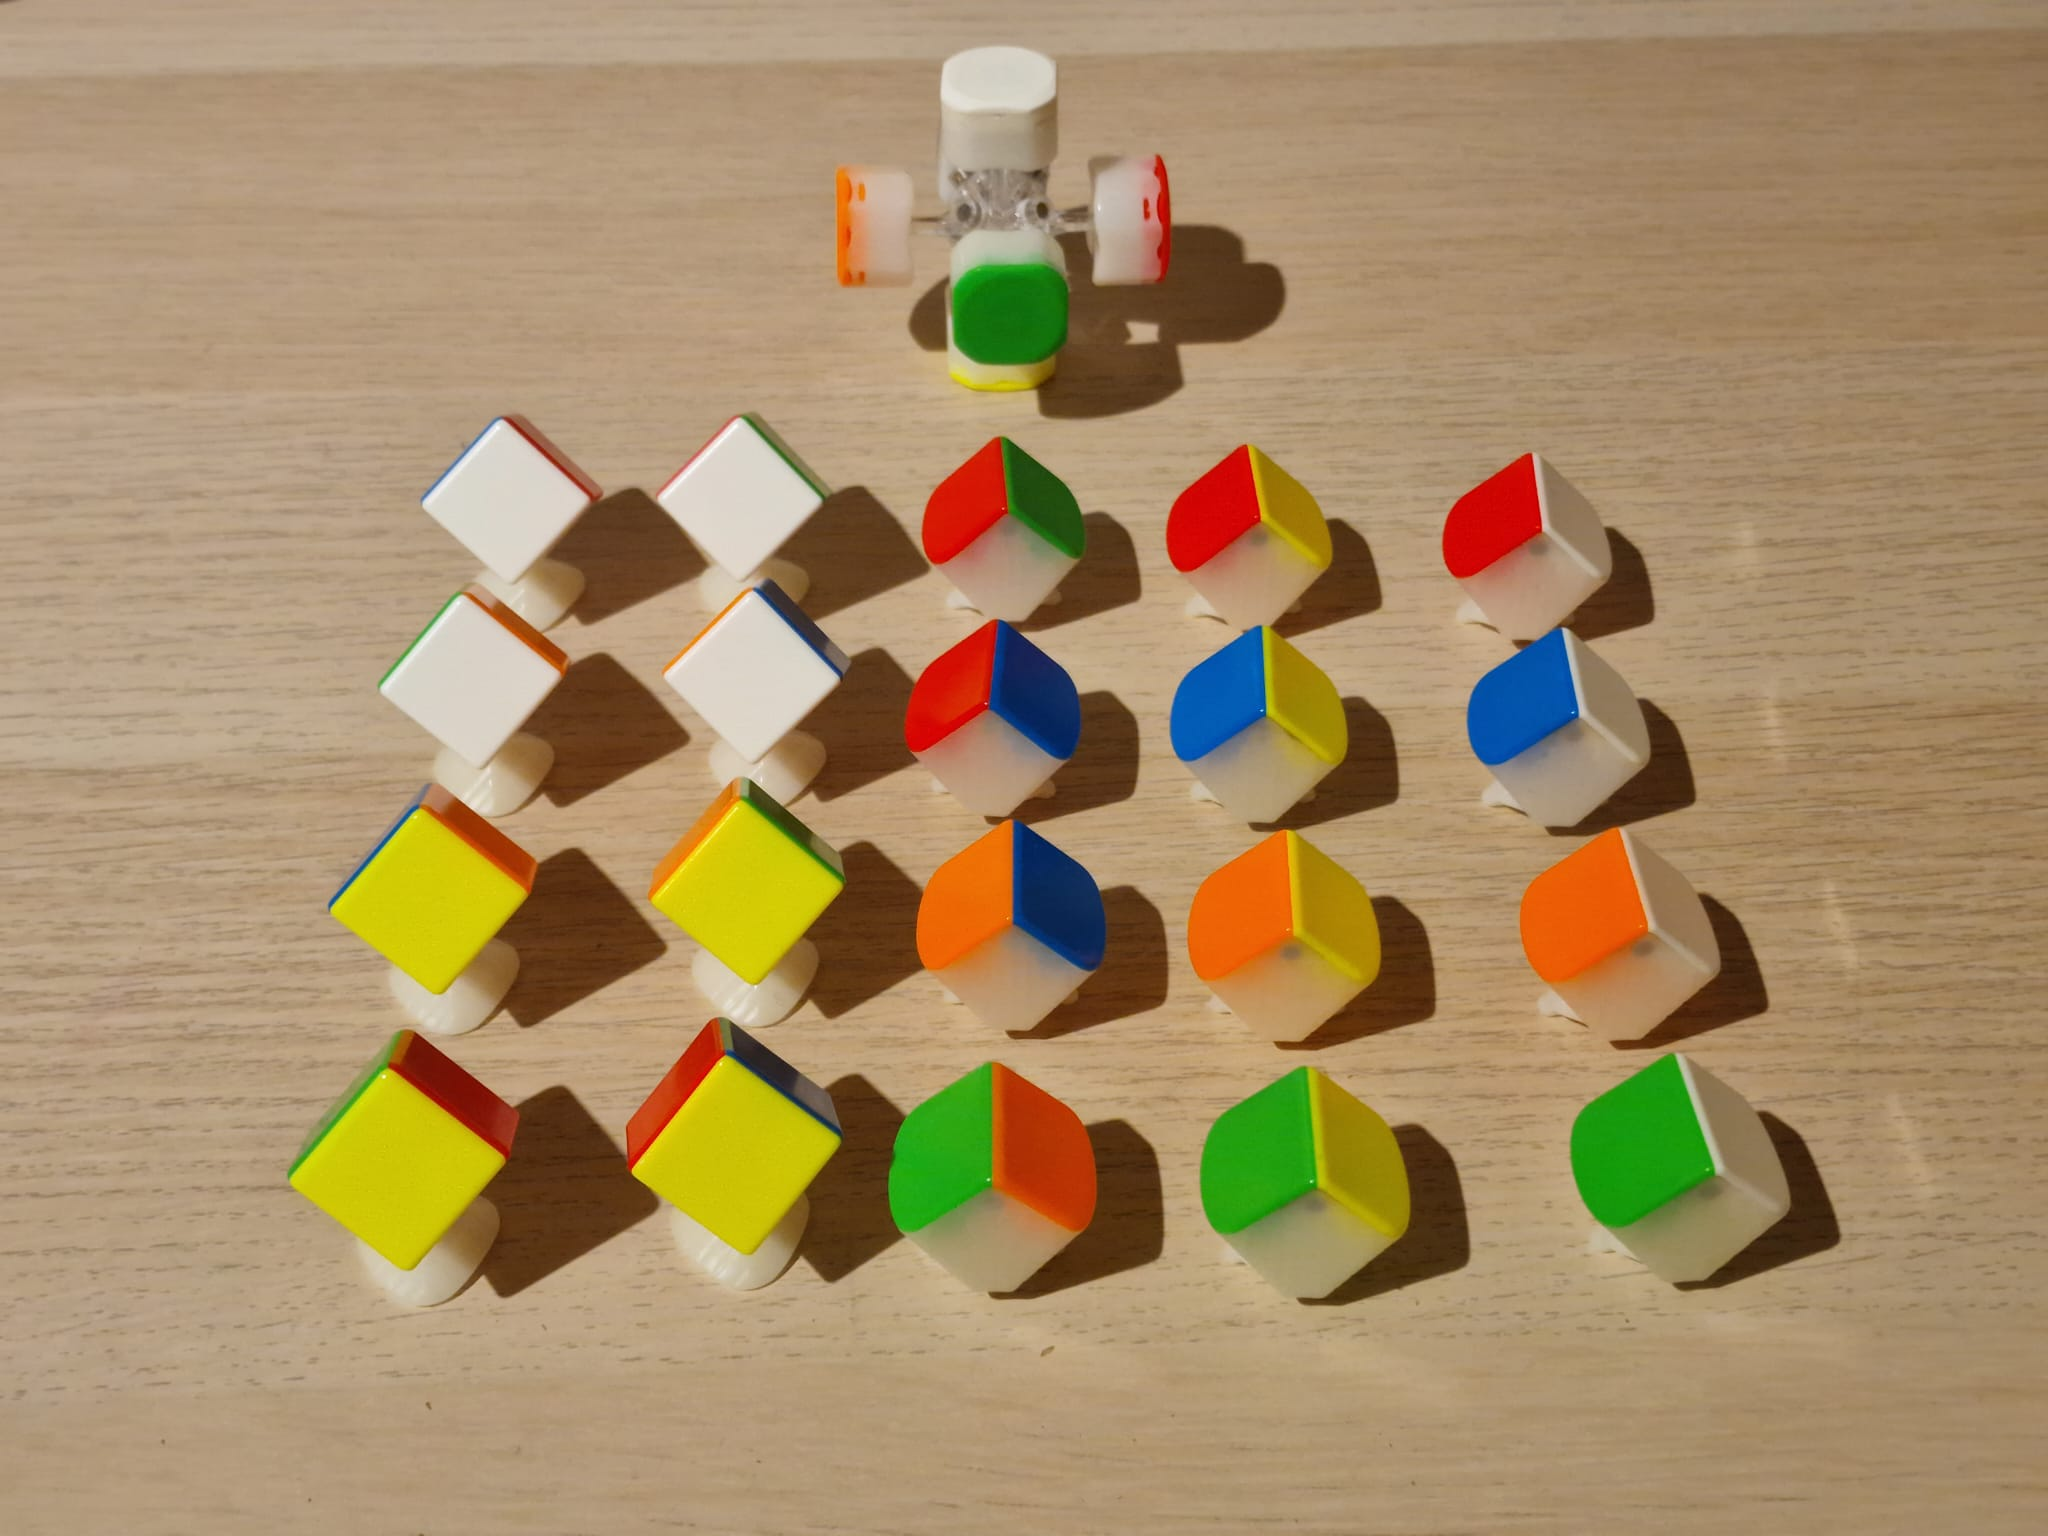
\includegraphics[width=10cm]{img/figures/cub-desmontat.jpg}
    \caption{Cub Desmuntat}
    \label{fig:cub-desmuntat}
\end{figure}

$$ \textrm{Nº Combinacions} = \frac{8!*3^8*12!*2^{12}}{12}= 43.252.003.274.489.856.000 $$